%%%%%%%%%%%%%%%%%%%%%%%%%%%%%%%%%
% Cerca la parola TODO all'interno di questo file per individuare ciò che devi personalizzare.
%%%%%%%%%%%%%%%%%%%%%%%%%%%%%%%%%
%
%
%


% Comandi per generare PDF-A2 con i relativi metadati 
\begin{filecontents*}[overwrite]{\jobname.xmpdata}
\Title{TODO Titolo del documento PDF}
\Author{TODO Nome autore}
\Language{it}
\Subject{TODO Breve frase descrittiva}
\Keywords{TODO\sep keyword2\sep keyword3}
\end{filecontents*}


%%%%%%%%%%%%%%%%%%%%%%%%%%%%%%%%%
%   PREAMBOLO DEL DOCUMENTO     %
%%%%%%%%%%%%%%%%%%%%%%%%%%%%%%%%%
\documentclass[a4paper,12pt,oneside,top=3cm,bottom=3cm,left=3.5cm,right=3.5cm,openright,reqno,table]{book}
% openany - fa iniziare i capitoli direttamente nella pagina successiva
% openright - fa iniziare i capitoli nella prima pagina destra disponibile 
% fleqn  - allinea le formule a sinistra anzichè centrarle
% leqno - dispone la numerazione delle formule sulla sinistra o destra
% reqno - dispone la numerazione delle formule sulla destra

% package fondamentali
\usepackage[T1]{fontenc}
\usepackage[utf8]{inputenc}
% se si realizza un documento in piu lingue bisogna istruire babel con
% [lingua_secondaria,lingua_principale]
\usepackage[italian]{babel}
\usepackage{colorprofiles}
\usepackage[colorlinks,hyperindex,pagebackref]{hyperref}
\hypersetup{
			citecolor=black,
			filecolor=black,
			linkcolor=black,
			urlcolor=black
}
% per generare il PDF-A2
\usepackage[a-2b,mathxmp]{pdfx}[2018/12/22]
\hypersetup{pdfstartview=}

% tutti i package sono specificati in un file a parte: packages.sty
\usepackage{packages}

% comandi personalizzati
\usepackage{utils}

% stile dei capitoli
\usepackage[SeSa]{fncychap}
% gli stili di capitolo disponibili sono i seguenti:
% SeSa, Sonny, Lenny, Rejne, Conny, PetersLenny, Bjornstrup, Glenn, Bjarne, Nicola

\linespread{1.5}

%%%%%%%%%%%%%%%%%%%%%%%%%%%%%%%%%
%   DOCUMENTO VERO E PROPRIO    %
%%%%%%%%%%%%%%%%%%%%%%%%%%%%%%%%%
\begin{document}

% frontespizio 
\begin{titlepage}
\changepage{}{}{}{-7.5 mm}{}{}{}{}{}
% parametri per cambiare le dimensioni di una singola pagina in ordine:
% {textheight}{textwidth}{evensidemargin}{oddsidemargin}{columnsep}
% {topmargin}{headheight}{headsep}{footskip}
% se voglio centrare la pagina devo mettere bindingoffset/2
% i primi 5 parametri posso usarli con \changetext


\begin{center}

\includegraphics [width=.15\columnwidth, angle=0]{logo-unisa}\\ % height
\vspace{0.5cm}
{\Large \scshape Università degli Studi di Salerno}\\
\vspace{0.5cm}
{\Large Dipartimento di Informatica}\\
\vspace{0.5cm}
{\Large Corso di Laurea Triennale in Informatica}\\
\vspace{1.5cm}
{\Large \scshape Tesi di Laurea} \\
\vspace{4cm}
{\Huge \bfseries Titolo della Tesi} \\
\vspace{4cm}

\begin{minipage}[t]{7cm}
\flushleft
{\large \textsc{Relatore}}

{\large Prof. Nome relatore} \\
{\large Dott. Nome tutor} \\
Università degli Studi di Salerno \\[0.25cm]
\end{minipage}
\hfill
\begin{minipage}[t]{7cm}
\flushright
{\large \textsc{Candidato}}

{\large \textbf{Nome Cognome}} \\
Matricola: 0123456789
\end{minipage}

\vspace{3cm}

{\small Anno Accademico YYYY-YYYY} %\\
%
%
\end{center}

\end{titlepage}


% sesalab
\begin{titlepage}
\nonumber
\null \vspace {\stretch{1}}
\begin{flushright}
{\textit{Questa tesi è stata realizzata nel} \hspace*{0.25cm}}
\\
\vspace{0.5cm}

\includegraphics[width=.40\columnwidth, angle=0]{logo-sesa}
\end{flushright}
\end{titlepage}


%dedica
\begin{titlepage}
\nonumber
\null \vspace {\stretch{1}}
	\begin{flushright}
%	\begin{verse}
\textit{Dedica o citazione} \\[5mm]
%	\end{verse}
	\end{flushright}
\end{titlepage}

% abstract
\renewcommand{\abstractname}{Abstract}
\begin{titlepage}
\begin{abstract}
%
Il testo dell'abstract qui...
%
\\[1cm]
\end{abstract}
\end{titlepage}

\frontmatter
% quello che segue è in numerazione romana e i capitoli non verranno numerati
% se non si vuole che compaia il numero di pagina basta usare il comando:
%\nonumber

% indici 
\phantomsection

% Il simbolo * serve per evitare che comapaia nell'indice

\tableofcontents
\clearpage

\addcontentsline{toc}{chapter}{Elenco delle Figure}
\listoffigures
\clearpage

\addcontentsline{toc}{chapter}{Elenco delle Tabelle}
\listoftables
\clearpage



\mainmatter
% quello che segue sarà in numerazione araba e i capitoli verranno numerati

% TODO inserire capitoli
\phantomsection
%\addcontentsline{toc}{chapter}{Introduzione}
\chapter{Introduzione}
\markboth{Introduzione}{}
% [titolo ridotto se non ci dovesse stare] {titolo completo}

\section{Motivazioni e Obiettivi} %\label{1sec:scopo}

\section{Risultati}

\section{Struttura della tesi}

\chapter{Esempio Capitolo} %\label{1cap:spinta_laterale}
% [titolo ridotto se non ci dovesse stare] {titolo completo}
%

%\begin{citazione}
%BREVE SPIEGAZIONE CONTENUTO CAPITOLO
%\end{citazione}

\section{Prima sezione}

\subsection{Prima sottosezione}

\paragraph{Primo paragrafo} Questa è una prova di un testo di un paragrafo.

The well known Pythagorean theorem $x^2 + y^2 = z^2$\footnote{\url{http://google.com}} was 
proved to be invalid \textbf{\textit{for other exponents}}. 

\textsc{com.java.xxx}

``Lorem ipsum''

Meaning the next equation has no integer solutions:

\[ x^n_m + y^n = z^n \]

\begin{figure}[h]
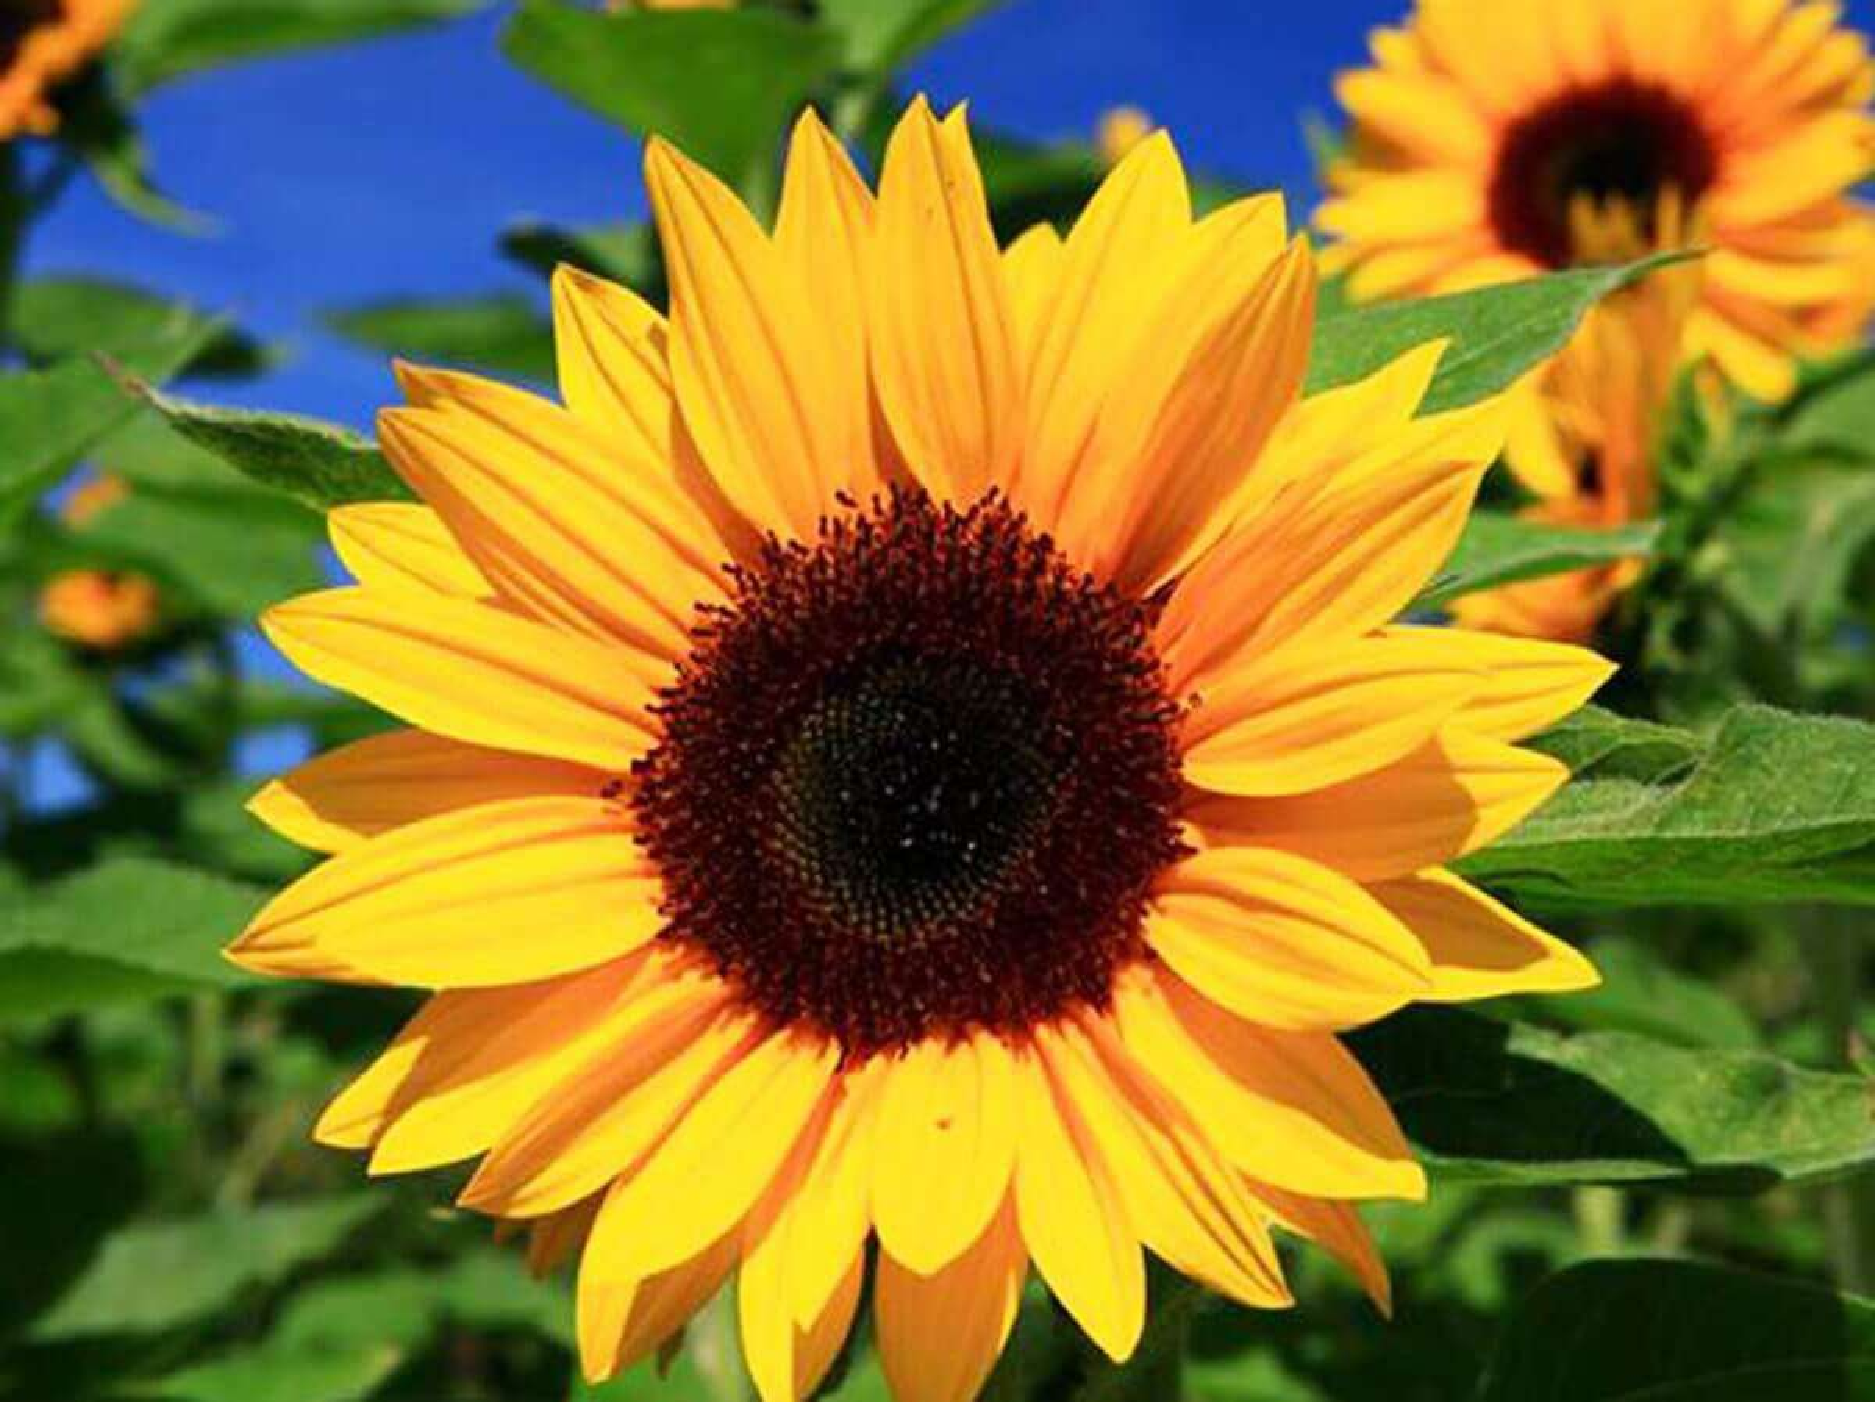
\includegraphics[width=3cm]{figure/picture.pdf}
\centering
\caption{Girasole piantato nel cortile del Dipartimento di Informatica.}
\end{figure}






\begin{table}
    \centering
    \caption{Questions to decide whether to conduct a MLR~\cite{garousi2019_mlr_guidelines}.}
    \vspace{1mm} % Adjust the height of the space between caption and tabular
    
    \rowcolors{1}{graytable}{white}
    \resizebox{\linewidth}{!}{
    \begin{tabular}{p{0.025\linewidth} p{0.875\linewidth} P{0.1\linewidth}}
        \toprule
        \rowcolor{black}
        \textbf{\textcolor{white}{\#}} & \textbf{\textcolor{white}{Question}} & \textbf{\textcolor{white}{Answer}}\\
        \bottomrule
        1 & Is the subject ``complex'' and not solvable by considering only the formal literature? & Yes\\
        2 & Is there a lack of volume or quality of evidence, or a lack of consensus of outcome measurement in the formal literature? & No\\
        3 & Is the contextual information important to the subject under study? & Yes\\
        4 & Is it the goal to validate or corroborate scientific outcomes with practical experiences? & Yes\\
        5 & Is it the goal to challenge assumptions or falsify results from practice using academic research or vice versa? & Yes\\
        6 & Would a synthesis of insights and evidence from the industrial and academic community be useful to one or even both communities? & Yes\\
        7 & Is there a large volume of practitioner sources indicating high practitioner interest in a topic? & Yes\\
        \bottomrule
        \rowcolor{white}
        \multicolumn{3}{p{\linewidth}}{\textit{\textbf{Note}: The possible answers to each question are ``Yes'' or ``No''. One or more ``Yes'' responses suggest that it could be useful to conduct a MLR.}}\\
    \end{tabular}
    }
    
    \label{table:motivations_MLR}
\end{table}









\begin{center}
\begin{table}[!h]
\begin{tabular}{||c c c ||}
 \hline
 Col1 & Col2 & Col3 \\ [0.5ex] 
 \hline\hline
 1 & 6 & 787 \\ 
 \hline
 2 & 7 & 5415 \\
 \hline
 3 & 545 & 7507 \\
 \hline
 4 & 545 & 7560 \\
 \hline
 5 & 88 & 6344 \\ [1ex] 
 \hline
\end{tabular}
\caption{Esempio di tabella}
\end{table}
\end{center}

The well known Pythagorean theorem $x^2 + y^2 = z^2$ was 
proved to be invalid for other exponents. 
Meaning the next equation has no integer solutions:

\[ x^n_m + y^n = z^n \]

\begin{minted}
[
frame=lines,
framesep=2mm,
baselinestretch=1.2,
bgcolor=LightGray,
fontsize=\footnotesize,
linenos
]
{python}
import numpy as np
    
def incmatrix(genl1,genl2):
    m = len(genl1)
    n = len(genl2)
    M = None #to become the incidence matrix
    VT = np.zeros((n*m,1), int)  #dummy variable
    
    #compute the bitwise xor matrix
    M1 = bitxormatrix(genl1)
    M2 = np.triu(bitxormatrix(genl2),1) 

    for i in range(m-1):
        for j in range(i+1, m):
            [r,c] = np.where(M2 == M1[i,j])
            for k in range(len(r)):
                VT[(i)*n + r[k]] = 1;
                VT[(i)*n + c[k]] = 1;
                VT[(j)*n + r[k]] = 1;
                VT[(j)*n + c[k]] = 1;
                
                if M is None:
                    M = np.copy(VT)
                else:
                    M = np.concatenate((M, VT), 1)
                
                VT = np.zeros((n*m,1), int)
    
    return M
\end{minted}

Questo è un elenco puntato
\begin{itemize}
    \item primo elemento
    \begin{itemize}
    \item primo sottoelemento
    \end{itemize}
    \item secondo elemento
    \item terzo elemento
\end{itemize}

Questo è un elenco numerato
\begin{enumerate}
    \item primo elemento
    \begin{enumerate}
    \item primo sottoelemento
    \end{enumerate}
    \item secondo elemento
    \item terzo elemento
\end{enumerate}

Questa è una frase che dice qualcosa, e deve essere supportata da una citazione.
Se gli autori sono più di due, scriviamo che Garousi et al. hanno detto qualcosa~\cite{garousi2019_mlr_guidelines}.
Se gli autori sono due, scriviamo che Bruegge e Dutoit hanno detto cose~\cite{bruegge2009object_se}.
Quest'altra frase dice qualcos'altro, ma non so in quale paper l'ho letta~\needcite.
Questa frase dice cose supportate da diverse pubblicazioni~\cite{casillo2022detecting,destefano2020splicing,giordano2022slr,iannone2022secret,lambiase2022fences,sellitto2022refactoring,pontillo2022static}.
In questa parte devo ricordarmi qualcosa\nb{devo ricordarmi di questa cosa}.

\revised{Questa parte del documento è stata modificata dopo che il relatore mi ha dato suggerimenti.}

Invece qui ho avuto dei feedback dal relatore, e devo ricordarmi di applicare i commenti. \feedback{aggiungi un paragrafo sulle research question}

\goal{Questo è l'obiettivo della tesi.}

\rqbox{1}{Quale è la nostra prima Research Question?}

\rqanswer{1}{Questa è la risposta alla prima RQ.}

\finding{1}{Questo è il primo finding che riportiamo tra i risultati.}

\takeaway{1}{Primo takeaway message.}


\chapter{Conclusioni} 

Le conclusioni qui...



\backmatter

% bibliografia in stile IEEE
\addcontentsline{toc}{chapter}{\bibname}
\bibliographystyle{IEEEtran}
\bibliography{references}

% ringraziamenti
\chapter*{Ringraziamenti}
\pagenumbering{gobble}
\fancyhf{}

Ringraziamenti qui...


% se hai intenzione di donare un albero tramite treedom
%\begin{titlepage}
\nonumber
\null \vspace {\stretch{1}}
\begin{flushright}
{\textit{Questa tesi ha contribuito a piantare un albero in Kenya tramite il progetto Treedom.}}
\\
\vspace{0.5cm}
{\footnotesize\url{https://www.treedom.net/it/user/sesalab/event/sesa-random-forest}}
\end{flushright}
\end{titlepage}


\end{document}

%%%%%%%%%%%%%%%%%%%%%%%%%%%%%%%%%